\documentclass[11pt]{article}
\usepackage[T1]{fontenc}
\usepackage[a4paper,margin=23mm]{geometry}
\usepackage{amsmath,amssymb,amsthm,booktabs,tikz}
\usetikzlibrary{positioning}
\usepackage[hidelinks]{hyperref}
\newtheorem{theorem}{Theorem}
\newtheorem{proposition}[theorem]{Proposition}
\newcommand{\Q}{\mathbb Q}
\newcommand{\Gal}{\operatorname{Gal}}
\newcommand{\Frob}{\operatorname{Frob}}
\newcommand{\RH}{\mathrm{RH}}
\newcommand{\tr}{\operatorname{tr}}
\title{Riemann hypotheses and cubic residues of 269 in arithmetic progressions}
\author{Mathematical research note produced by GPT-6.2 Astra}
\date{22 November 2026}
\begin{document}
\maketitle
\begin{abstract}
For the pure cubic field generated by the cube root of 269, the nonabelian
Artin factor has a concrete prime coefficient. It measures whether 269 is
a cube at primes congruent to one modulo three. We give equivalent Riemann
hypotheses for its Dirichlet twists, two families of Dedekind zeta functions,
and square-root cancellation of these coefficients at primes that are
one modulo a fixed modulus. Applying Alp\"oge's Landau-window theorem to
the product of the twists gives a one-sided test on a sequence of long
intervals using this progression alone. We compute the mean-square error of a predictor
that uses a fixed congruence class. The same obstruction survives after adjoining
all splitting data for the cube root of 269 if the tested radicand is changed
to 2. These are deductions from classical Artin formalism and Chebotarev.
\end{abstract}

\section{The prime coefficient}
Let $F=\Q(\sqrt[3]{269})$, $K=\Q(\zeta_3)$ and $E=FK$.
The cubic is Eisenstein at 269. Its discriminant has square class $-3$,
so $G=\Gal(E/\Q)=S_3$. Let $\rho$ be the two-dimensional summand of the
permutation representation on its roots and $\eta$ the sign character.
At each prime $p\nmid 3\cdot269$ put
\[
t(p)=\#\{x\in\mathbb F_p:x^3=269\}-1 .
\]
Then $t(p)=\tr \rho(\Frob_p)$. For the Artin factorization of a
non-Galois cubic field see Shankar--S\"odergren--Templier~\cite{DS}.
The splitting of the cubic gives the entire table.
\begin{center}
\begin{tabular}{llrr}
\toprule
Congruence & Cubic condition & Frobenius type & $t(p)$\\
\midrule
$p\equiv 2\bmod3$ & unique root & $(12)$ & $0$\\
$p\equiv 1\bmod3$ & $269^{(p-1)/3}\equiv1\bmod p$ & $1$ & $2$\\
$p\equiv 1\bmod3$ & $269^{(p-1)/3}\not\equiv1\bmod p$ & $(123)$ & $-1$\\
\bottomrule
\end{tabular}
\end{center}
The primes 7 and 37 are both 7 modulo 30. The cubic has no root modulo 7
and has the three roots $7,33,34$ modulo 37. The sign character takes the
same value at these primes.

\section{The equivalences at each modulus}
Fix $M\ge1$, $A=\Q(\zeta_M)$ and $D=\Gal(A/\Q)$. All characters of $D$
below are viewed as Galois characters. Their $L$-functions use the
primitive local factors, including the inertia invariants at ramified
places. When we form prime sums we omit primes dividing $3\cdot269M$.
By RH for an individual function we mean that all its zeros in
$0<\Re s<1$ lie on $\Re s=1/2$.

\begin{theorem}\label{t:first}
Assume RH for the Dirichlet factors $L(s,\chi)$ and $L(s,\eta\chi)$
for all $\chi\in\widehat D$, interpreting the trivial factor as
$\zeta_{\Q}$. The following statements are equivalent:
\begin{enumerate}
\item $\RH$ holds for $L(s,\rho\otimes\chi)$ for every $\chi\in\widehat D$.
\item $\RH$ holds for $\zeta_{FA}$.
\item $\RH$ holds for $\zeta_{EA}$.
\item For every $a\in(\mathbb Z/M)^\times$ and every $\epsilon>0$,
\[
 \sum_{\substack{p\le x,\ p\equiv a\ (M)\\p\equiv1\ (3)\\p\nmid3\cdot269M}}
       \left(3\mathbf1_{269^{(p-1)/3}\equiv1\ (p)}-1\right)\log p
       =O_{M,\epsilon}(x^{1/2+\epsilon}).
\]
\item The bound in (4) holds for $a=1$ for every $\epsilon>0$.
\end{enumerate}
The constants concern a fixed modulus. For $M=1$ this gives exactly
the original cubic Artin factor, $\zeta_F/\zeta_{\Q}$.
\end{theorem}
\begin{proof}
The permutation representation of $F$ is $1+\rho$. Since $A/\Q$ is
Galois and $F\cap A=\Q$, the permutation representation of $FA$
is $(1+\rho)\otimes{\rm reg}_D$. Write $d=[E\cap A:\Q]$, which
is one or two because $K$ is the maximal abelian subfield of $E$.
In the action on the pairs of embeddings of $E,A$, each orbit is free
under $\Gal(EA/\Q)$ and there are $d$ orbits. The regular representation
of $S_3$ has character $1+\eta+2\rho$. Artin formalism gives
\begin{align*}
\zeta_{FA}(s)&=\prod_{\chi\in\widehat D}L(s,\chi)L(s,\rho\otimes\chi),\\
\zeta_{EA}(s)^d&=\prod_{\chi\in\widehat D}L(s,\chi)L(s,\eta\chi)
                                    L(s,\rho\otimes\chi)^2 .
\end{align*}
All factors are holomorphic in the open strip. Indeed
$\rho=\operatorname{Ind}_{G_K}^{G_{\Q}}\nu$ for a nontrivial cubic
character of $E/K$, and twisting by $\chi$ preserves irreducibility.
Its twist is induced from the nontrivial finite-order Hecke character
$\nu\chi|_{G_K}$. Hecke's holomorphy theorem applies. Thus zeros of the
factors in the strip contribute with their actual positive multiplicities.
This proves equivalence of the first three statements.

Under (3) the effective Chebotarev theorem for $EA/\Q$ gives, for each
conjugacy class, the main term plus $O_{EA}(x^{1/2}\log^2(2x))$ for its
logarithmically weighted prime sum \cite{LO}. Over each given element
of $D$, the trace $t$ has mean zero: $\Gal(EA/A)$ projects to $S_3$
or $A_3$ and $\rho$ has no invariants under either. Summing the class
estimates gives (4).

For the converse, (4) implies (5). Put
$P_M(s)=\prod_{\chi\in\widehat D} L(s,\rho\otimes\chi)$.
At an unramified prime its logarithmic-derivative prime sum has
coefficient $t(p)\sum_\chi\chi(p)$, which is $\varphi(M)t(p)$ if
$p\equiv1\bmod M$ and zero otherwise, with weight $\log p$.
The total contribution of prime powers of exponent at least two is
$O_M(\sqrt{x}\log^2(2x))$, since the underlying traces are bounded
by $2\varphi(M)$. The finitely many omitted primes contribute
$O_M(\log(2x))$. Thus (5) bounds the partial sums of the coefficients
of $-P'_M/P_M$. Partial summation gives a holomorphic
continuation of this series to every half-plane $\Re s>1/2+\epsilon$.
It agrees with the logarithmic derivative on $\Re s>1$, so the product
has no zero in $\Re s>1/2$. Its factors are entire. The
functional equation reflects any zero of an individual factor
on the left to the right for the conjugate twist, which is also in the
family. This proves (1).
\end{proof}
The choice of residue class matters. For $M=3$ the class $a=2$
has $t(p)=0$ identically and imposes no condition at all. The
class $a=1$ retains the unweighted product of the entire factors.

\section{A one-sided test on arbitrarily late intervals}
Here is a consequence of Alp\"oge's general Landau-window theorem
\cite{A}. The workshop applied it to a single cubic character in AM-H04.
We apply the same analytic input to the product $P=P_M$ and remove the
higher prime powers from the observed statistic.
Define $D(s)=P'(s)/P(s)$ and, in $\Re s>1$, write
$-D(s)=\sum b(n)n^{-s}$. Define $b_1(p)=\varphi(M)t(p)\log p$
when $p\nmid3\cdot269M$ and $p\equiv1\bmod M$, and put $b_1(n)=0$
elsewhere. Write $h=b-b_1$. Set
\[
C_M=D(1)+\sum_{n\ge1}\frac{h(n)}n,\qquad
R_M(y)=\sum_{p\le y} b_1(p)(y/p-1)+y C_M .
\]
These definitions use the full primitive Euler factors in $P$. Its value
at one is nonzero by the simple-pole residues of
$P=\zeta_{FA}/\zeta_A$. The correction series is absolutely convergent.

\begin{proposition}\label{p:window}
Fix $\delta>0$. Under the Dirichlet hypotheses of Theorem~\ref{t:first},
each of its equivalent assertions is equivalent to the following one.
For every $1/2<\theta<1$ there is $C_\theta>0$ such that for
arbitrarily large $Y$,
\[
                  R_M(y)\le C_\theta y^\theta
                  \qquad(Y\le y\le Y^{1+\delta}).
\]
In this implication from the window to the twisted zero statements,
the arithmetic input yet to be proved is the displayed inequality.
\end{proposition}
\begin{proof}
The omitted coefficients $h(n)$ occur at higher powers of primes and
the first powers of the finitely many bad primes. The eigenvalues at
a prime power on inertia invariants have absolute value at most one,
hence $\sum_{n\le y}|h(n)|=O_M(\sqrt{y}\log^2(2y))$.
Abel summation gives the same upper bound for
$y\sum_{n>y}|h(n)|/n$. For the full ramp
\[
 G(y)=\sum_{n\le y}b(n)(y/n-1)+yD(1)
\]
it follows that $G(y)-R_M(y)=-\sum_{n\le y}h(n)-y\sum_{n>y}h(n)/n
=O_M(\sqrt{y}\log^2(2y))$. In particular the bound transfers from
$R_M$ to $G$ on every proposed interval.

Put $g(u)=G(e^u)$ and let $Z$ be the zeros of $P$ with positive real
part. Its real finite-image representation is
$\rho\otimes{\rm reg}_D$, so $g$ is real, continuous and
$|g(u)|=O_M(e^{2u})$ for $u\ge0$. Direct termwise integration gives
\[
\int_1^\infty G(y)y^{-s-1}\,dy
     =\frac{sD(1)-D(s)}{s(s-1)}\qquad(\Re s>1).
\]
The apparent pole at one is removable. In the positive half-plane
the transform is holomorphic off the locally discrete set $Z$.
A zero $z$ of multiplicity $m$ yields a simple pole of residue
$m/[z(1-z)]$, positive at each real zero there. These are exactly
the pole and growth data in the cited theorem. On $U\le u\le(1+\delta)U$
the upper majorant $C e^{\theta u}$ has weighted integral $C\delta U$,
which is at most $e^{\eta U}$ for every fixed $\eta>0$ and sufficiently
large such $U=\log Y$. The theorem gives $\Re z\le\theta$ for every
$z\in Z$. Let $\theta$ decrease to $1/2$ and use the functional equations
as in Theorem~\ref{t:first}.

Conversely the RH assumptions give
$B_1(y)=\sum_{p\le y}b_1(p)=O_M(\sqrt{y}\log^2(2y))$ by effective
Chebotarev. Hence $\sum b_1(p)/p$ converges and equals $-C_M$
by taking $s\downarrow1$ in the logarithmic derivative. It follows
that $R_M(y)=-B_1(y)-y\sum_{p>y}b_1(p)/p
=O_M(\sqrt{y}\log^2(2y))$, proving the assertion on every interval.
\end{proof}
The exact centering constant matters: changing it by $c$ adds $cy$.
In particular a downward bias in this constant could force a one-sided
inequality with no arithmetic content. The reduction does not estimate
$C_M$ to the accuracy that a numerical test on growing windows would need.

\section{What congruence information retains}
\begin{theorem}\label{t:error}
For every function $b:(\mathbb Z/M)^\times\to\mathbb C$,
\[
\lim_{x\to\infty}\frac1{\pi(x)}
 \sum_{\substack{p\le x\\p\nmid3\cdot269M}}|t(p)-b(p\bmod M)|^2
 =1+\frac1{\varphi(M)}\sum_{a\in(\mathbb Z/M)^\times}|b(a)|^2.
\]
Consequently the infimum of the squared error over all fixed moduli
and all predictors on their reduced residue classes is exactly one.
\end{theorem}
\begin{proof}
Chebotarev without any RH identifies the limiting average with uniform
group average over $\Gal(EA/\Q)$. On each fibre of the restriction to
$D$ the mean of $t$ vanishes by the averaging projector in the preceding
proof. Its mean square is $\langle\chi_\rho,\chi_\rho\rangle=1$ by
irreducibility. Expanding the square proves the identity. The zero
predictor attains equality.
\end{proof}
This computation also rules out approximation in the Hilbert-space
closure of all such fixed-modulus predictors for this limiting mean-square
norm. The order of limits matters. It gives no bound on a modulus
chosen afresh as a function of the sample cutoff $x$, and it rules out no
analytic proof using many auxiliary characters with quantitative estimates.

\begin{proposition}\label{p:2}
Replace $269$ by $2$ in the definition of $t$, writing $t_2$ for the
result and omitting all primes dividing $2\cdot3\cdot269M$.
Allow a predictor to use the \emph{full} Frobenius conjugacy class
in $E\Q(\zeta_M)$ for any fixed $M$. Its mean squared error is again
$1$ plus its own mean squared size.
\end{proposition}
\begin{proof}
Let $E'=K(\sqrt[3]{2})$. In $K^\times/K^{\times3}$, the classes of
$2$ and $269$ are independent: each is an inert prime and valuations
there give the two independent coordinate tests modulo three. Kummer
theory gives $\Gal(EE'/K)=C_3^2$. Complex conjugation inverts both
factors and hence the commutator subgroup of $\Gal(EE'/\Q)$ is all
of $C_3^2$. Its maximal abelian subfield is $K$.
Consequently $\Gal(EE'\Q^{\rm ab}/\Q^{\rm ab})=C_3^2$, and
the subgroup fixing $E\Q^{\rm ab}$ maps onto $\Gal(E'/K)=C_3$.
The standard character for $E'$ has no invariant vector on this
subgroup. The same is true on the larger subgroup fixing $E\Q(\zeta_M)$.
In the finite quotient for $EE'A$, use the same fibre projector and
Chebotarev as in Theorem~\ref{t:error}.
\end{proof}
In particular the trace for $E'$ lies outside the finite character
identities supplied by all Dirichlet twists of this one cubic field,
even allowing their tensor products. This is a statement about
representations and observable prime data. It gives no logical
independence between the Riemann hypotheses for the two fields.

\begin{figure}[ht]
\centering
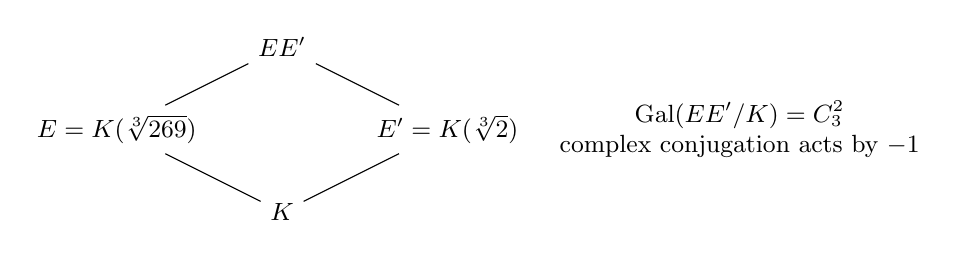
\begin{tikzpicture}[font=\small, every node/.style={align=center}]
\node (base) at (0,0) {$K$};
\node (e) at (-2.1,1.05) {$E=K(\sqrt[3]{269})$};
\node (f) at (2.1,1.05) {$E'=K(\sqrt[3]{2})$};
\node (ef) at (0,2.1) {$EE'$};
\draw (base)--(e)--(ef)--(f)--(base);
\node[right] at (3.4,1.05) {$\Gal(EE'/K)=C_3^2$\\
complex conjugation acts by $-1$};
\end{tikzpicture}
\caption{Both cubic directions survive abelian base change. Fixing the
left field leaves the right-hand cubic direction nontrivial, as used in
Proposition~\ref{p:2}. Every edge has degree three.}
\end{figure}
\begin{thebibliography}{9}
\bibitem{A} L. Alp\"oge, formal source for the Dirichlet Riemann hypothesis,
\emph{LandauTheorems/landauWindow.lean}, theorem
\texttt{Deduction.landau\_window}, lines 83--84;
\emph{LandauZeroFreeCriterion.lean}, structures
\texttt{PoleData} and \texttt{WindowHypU}. Source snapshot
\href{https://github.com/CocoSgt/riemann-hypothesis-lean/tree/7cbf7a0c32fca1badf05931879a37c3f8a2b03b4/src/Development/AutomorphicArithmetic/DedekindLFunctions}
{7cbf7a0}, dated November 2026. The generic analytic theorem is an input.
\bibitem{DS} A. Shankar, A. S\"odergren and N. Templier,
\emph{Central values of zeta functions of non-Galois cubic fields},
Inventiones Mathematicae \textbf{243}, 33--116, section 1.1,
\url{https://doi.org/10.1007/s00222-025-01373-6}.
\bibitem{LO} J. C. Lagarias and A. M. Odlyzko, Effective versions of the
Chebotarev density theorem, in \emph{Algebraic Number Fields},
Academic Press, 1977, 409--464, Theorem 1.1.
\end{thebibliography}
\end{document}
